% =============================================================================
% PyCore + ExCore — system architecture overview for the research paper
% =============================================================================
% Build (from this directory):
%   pdflatex architecture_overview.tex && pdflatex architecture_overview.tex
% Requires: article, tikz, booktabs, hyperref, geometry, microtype, xcolor
% =============================================================================
\documentclass[11pt,a4paper]{article}

\usepackage[margin=0.9in]{geometry}
\usepackage[expansion=false]{microtype}
\usepackage{booktabs}
\usepackage{tabularx}
\usepackage{graphicx}
\usepackage{xcolor}
\usepackage{hyperref}
\usepackage{amsmath}
\usepackage{amssymb}
\usepackage{enumitem}
\usepackage{float}
\usepackage{tikz}
\usetikzlibrary{arrows.meta,positioning,fit,calc,shapes.geometric,shapes.multipart,backgrounds}

\hypersetup{
  colorlinks=true,
  linkcolor=black,
  urlcolor=blue!50!black,
  citecolor=black
}

% Palette — cool slate / teal (avoid purple / cream / newspaper defaults)
\definecolor{pyfill}{RGB}{232,242,248}
\definecolor{pyborder}{RGB}{36,90,120}
\definecolor{exfill}{RGB}{236,245,236}
\definecolor{exborder}{RGB}{45,110,70}
\definecolor{memfill}{RGB}{248,242,230}
\definecolor{memborder}{RGB}{140,100,40}
\definecolor{toolfill}{RGB}{245,240,248}
\definecolor{toolborder}{RGB}{90,70,110}
\definecolor{roadfill}{RGB}{250,248,240}
\definecolor{roadborder}{RGB}{120,90,40}
\definecolor{arrowc}{RGB}{50,50,50}

\title{PyCore + ExCore: System Architecture\\
\large Component map for the research paper}
\author{PyCore systems notes\\
\texttt{docs/paper/systems/architecture\_overview.tex}}
\date{August 2026}

\begin{document}
\maketitle

\begin{abstract}
PyCore is a research CPU whose native ISA is a filtered CPython~3.14 bytecode
subset, implemented as a multi-cycle SystemVerilog hart with tagged 132-bit
architectural values.
ExCore is a companion RV32 multicycle hart that services \emph{recoverable}
container and helper traps in firmware under an exclusive shared-dmem ownership
protocol.
Together they form an asymmetric two-core machine: a bytecode fast path in
hardware, and a firmware completion path that finishes the trapped semantic
effect rather than merely retrying.
This note decomposes the system into the components we propose as primary
sections of the upcoming research paper, and provides an architecture diagram
that places those components in relation to one another and to the roadmap
(BIOS boot, on-device tokenizer, self-hosted \texttt{compile()}).
\end{abstract}

\tableofcontents
\newpage

% =============================================================================
\section{Thesis in one paragraph}
% =============================================================================

Executing CPython bytecode as a first-class ISA forces microarchitecture to
absorb language semantics that conventional CPUs push into compilers and runtimes:
typed values, open-addressed dicts, call binding, exception tables, and
iterator protocols.
PyCore keeps the high-frequency typed paths in a multi-cycle bytecode hart;
ExCore absorbs capacity-changing and $O(n)$ container work (and selected helpers)
behind a mailbox and memory grant, under a \textbf{complete-the-semantic-effect}
contract.
The research claim is that this split---tagged bytecode ISA + asymmetric
exception core + CPython image fidelity---is a practical way to study and
accelerate Python-shaped workloads without reimplementing all of CPython's
object protocol in silicon.

% =============================================================================
\section{Paper component map}
% =============================================================================

Table~\ref{tab:sections} is the proposed section skeleton.
Each row is a \emph{paper-worthy} component: novel enough to stand alone, and
load-bearing enough that later sections depend on it.
Sibling systems notes already exist for some rows (e.g.\ the CALL FSM);
others should grow into their own notes as they stabilize.

\begin{table}[ht]
\centering
\small
\begin{tabular}{@{}clp{0.58\textwidth}@{}}
\toprule
\# & Paper section & Core idea \\
\midrule
1 & Tagged bytecode ISA &
  Native CPython~3.14 units as instructions; 132-bit
  $\{\mathrm{tag}[3{:}0],\mathrm{value}[127{:}0]\}$ entries co-located in the RF. \\
2 & PyCore microarchitecture &
  Multi-cycle, non-pipelined control
  (\texttt{S\_FETCH}${\to}$\texttt{DECODE}${\to}$\texttt{EXEC}${\to}$\texttt{MEM}${\to}$\texttt{WB})
  plus specialized FSMs (\texttt{S\_CONTAINER}, \texttt{S\_CALL}, trap marshal). \\
3 & Tag-routed execute fabric &
  Tag decode, BOOL/INT/FLOAT promotion, INT ALU / mul / div / FPU / complex,
  trap policy for unsafe tags. \\
4 & Object \& container model &
  Bump heap; stable LIST/DICT/SET objects with relocatable buffers;
  \texttt{OBJECT} kinds; contamination bit for bulk ops. \\
5 & Asymmetric two-core design &
  Bytecode hart + RV32 ExCore; recoverable vs fatal trap taxonomy;
  private IMEMs, shared dmem. \\
6 & Ownership \& completion protocol &
  Mailbox handshake; exclusive memory grant; COMPLETED / RETRY / FATAL;
  ``finish the effect, don't just resize.'' \\
7 & Container co-design &
  Hash/probe/eq and spare-capacity append on PyCore;
  grow / extend / mid-delete / bulk merge on ExCore. \\
8 & CALL FSM \& frames &
  Shared binder for CALL / CALL\_KW / CALL\_FUNCTION\_EX;
  dmem frame stack; method / builtin / type arms. \\
9 & Exceptions \& iteration &
  Exception-table field on code objects; exc-info stack;
  GET\_ITER / FOR\_ITER; protocol CALL pause/resume. \\
10 & Image fidelity \& tooling &
  \texttt{compile()} graph $\to$ tagged imem/dmem; boot record;
  fidelity boundary (bytecode-identical, layout not C-struct). \\
11 & Firmware builtins \& ROM &
  ROM-seeded pure-Python builtins; LEGB-B;
  hardware \texttt{BI\_*} fast paths vs CODE\_OBJECT frames. \\
12 & Roadmap: self-hosting &
  Code ROM+RAM, BIOS, \texttt{exec}/\texttt{eval}, tokenizer (Plan~1);
  parser/AST/codegen/\texttt{compile()} (Plan~2). \\
\bottomrule
\end{tabular}
\caption{Proposed research-paper sections derived from the as-built system
and documented direction.}
\label{tab:sections}
\end{table}

\subsection{Why these cuts (not a file tree)}

A paper organized as ``RTL modules we happen to have'' would bury the
interesting claims.
The cuts above follow \emph{research seams}:

\begin{itemize}[leftmargin=1.2em,itemsep=0.25em]
  \item \textbf{ISA vs microarchitecture} --- tags and opcodes are the contract;
        the FSM is how we implement them.
  \item \textbf{Language semantics in hardware vs firmware} --- the ExCore
        boundary is the central systems contribution.
  \item \textbf{Fidelity vs completeness} --- image tooling locks bytecode
        fidelity today; Plans~1--2 describe the path to host independence.
  \item \textbf{Hot path vs protocol path} --- CALL/containers stay native;
        \texttt{\_\_iter\_\_}/\texttt{\_\_next\_\_} and exception handlers reuse
        the same CALL machinery via pause/resume.
\end{itemize}

% =============================================================================
\section{System architecture diagram}
% =============================================================================

Figure~\ref{fig:system} is the single overview figure intended for the paper's
architecture section.
Solid arrows are data/control paths in the as-built two-core top
(\texttt{pycore\_excore\_system}).
Dashed boxes are roadmap surfaces that already have planning contracts
(\texttt{planning/code\_loading\_bios\_tokenizer\_plan.md},
\texttt{planning/native\_compiler\_plan.md}).

\begin{figure}[H]
\centering
\resizebox{\textwidth}{!}{%
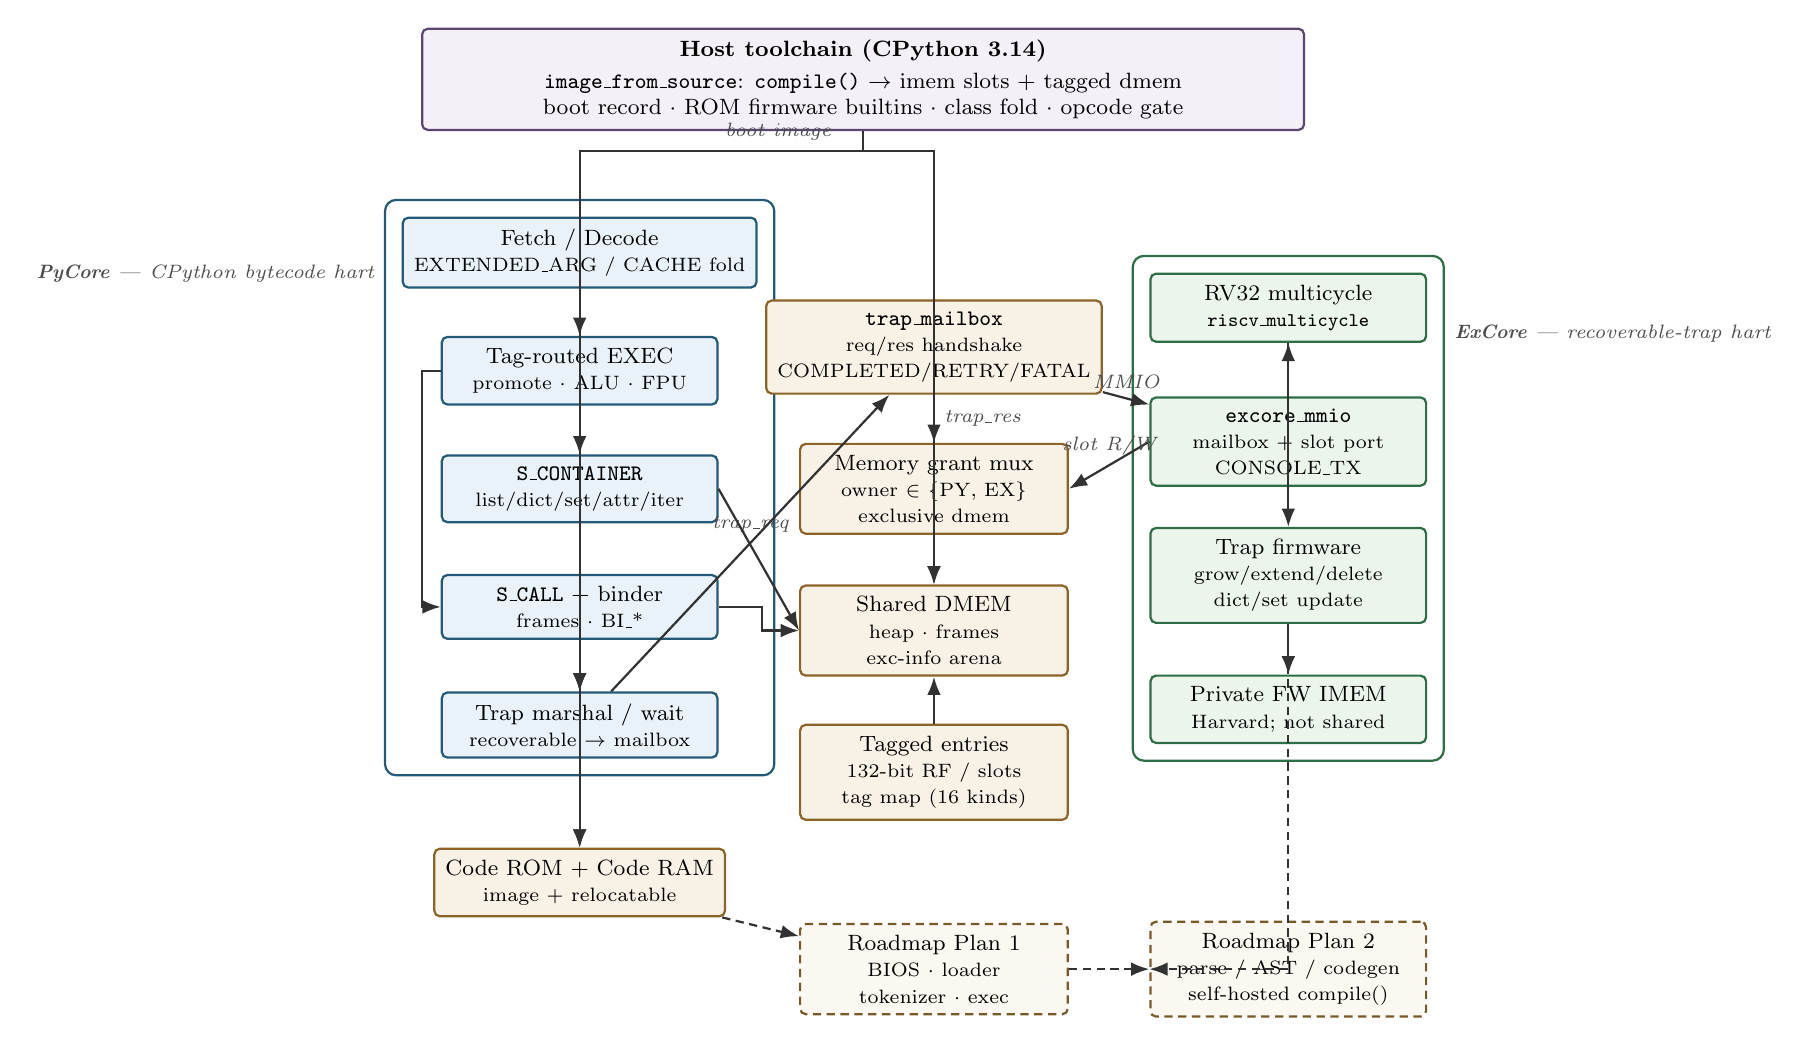
\begin{tikzpicture}[
  font=\footnotesize,
  >=Latex,
  box/.style={
    draw, rounded corners=2pt, align=center,
    inner sep=4pt, thick
  },
  py/.style={box, fill=pyfill, draw=pyborder, text=black},
  ex/.style={box, fill=exfill, draw=exborder, text=black},
  mem/.style={box, fill=memfill, draw=memborder, text=black},
  tool/.style={box, fill=toolfill, draw=toolborder, text=black},
  road/.style={box, fill=roadfill, draw=roadborder, text=black,
    densely dashed},
  grp/.style={draw, rounded corners=4pt, inner sep=6pt, thick},
  arr/.style={-{Latex}, thick, color=arrowc},
  sarr/.style={-{Latex}, thick, densely dashed, color=arrowc},
  lab/.style={font=\scriptsize\itshape, text=black!70}
]

% ---- Host tooling (top) ----
\node[tool, minimum width=11.2cm] (host) at (0, 10.4) {%
  \textbf{Host toolchain (CPython 3.14)}\\[2pt]
  \texttt{image\_from\_source}: \texttt{compile()} $\to$ imem slots + tagged dmem\\
  boot record $\cdot$ ROM firmware builtins $\cdot$ class fold $\cdot$ opcode gate};

% ---- PyCore cluster ----
\node[py, minimum width=3.5cm] (fetch) at (-3.6, 8.2) {%
  Fetch / Decode\\
  {\scriptsize EXTENDED\_ARG / CACHE fold}};
\node[py, minimum width=3.5cm] (exec) at (-3.6, 6.7) {%
  Tag-routed EXEC\\
  {\scriptsize promote $\cdot$ ALU $\cdot$ FPU}};
\node[py, minimum width=3.5cm] (cont) at (-3.6, 5.2) {%
  \texttt{S\_CONTAINER}\\
  {\scriptsize list/dict/set/attr/iter}};
\node[py, minimum width=3.5cm] (call) at (-3.6, 3.7) {%
  \texttt{S\_CALL} + binder\\
  {\scriptsize frames $\cdot$ BI\_*}};
\node[py, minimum width=3.5cm] (trapm) at (-3.6, 2.2) {%
  Trap marshal / wait\\
  {\scriptsize recoverable $\to$ mailbox}};

\node[grp, draw=pyborder, fit=(fetch)(exec)(cont)(call)(trapm),
  label={[lab]above left:\textbf{PyCore} --- CPython bytecode hart}] (pygrp) {};

% ---- Shared memory / transport (center) ----
\node[mem, minimum width=3.4cm] (mailbox) at (0.9, 7.0) {%
  \texttt{trap\_mailbox}\\
  {\scriptsize req/res handshake}\\
  {\scriptsize COMPLETED/RETRY/FATAL}};
\node[mem, minimum width=3.4cm] (grant) at (0.9, 5.2) {%
  Memory grant mux\\
  {\scriptsize owner $\in$ \{PY, EX\}}\\
  {\scriptsize exclusive dmem}};
\node[mem, minimum width=3.4cm] (dmem) at (0.9, 3.4) {%
  Shared DMEM\\
  {\scriptsize heap $\cdot$ frames}\\
  {\scriptsize exc-info arena}};
\node[mem, minimum width=3.4cm] (tags) at (0.9, 1.6) {%
  Tagged entries\\
  {\scriptsize 132-bit RF / slots}\\
  {\scriptsize tag map (16 kinds)}};

% ---- ExCore cluster ----
\node[ex, minimum width=3.5cm] (rv) at (5.4, 7.5) {%
  RV32 multicycle\\
  {\scriptsize \texttt{riscv\_multicycle}}};
\node[ex, minimum width=3.5cm] (mmio) at (5.4, 5.8) {%
  \texttt{excore\_mmio}\\
  {\scriptsize mailbox + slot port}\\
  {\scriptsize CONSOLE\_TX}};
\node[ex, minimum width=3.5cm] (fw) at (5.4, 4.1) {%
  Trap firmware\\
  {\scriptsize grow/extend/delete}\\
  {\scriptsize dict/set update}};
\node[ex, minimum width=3.5cm] (fimem) at (5.4, 2.4) {%
  Private FW IMEM\\
  {\scriptsize Harvard; not shared}};

\node[grp, draw=exborder, fit=(rv)(mmio)(fw)(fimem),
  label={[lab]above right:\textbf{ExCore} --- recoverable-trap hart}] (exgrp) {};

% ---- Bottom memories / roadmap ----
\node[mem, minimum width=3.5cm] (imem) at (-3.6, 0.2) {%
  Code ROM + Code RAM\\
  {\scriptsize image + relocatable}};
\node[road, minimum width=3.4cm] (bios) at (0.9, -0.9) {%
  Roadmap Plan~1\\
  {\scriptsize BIOS $\cdot$ loader}\\
  {\scriptsize tokenizer $\cdot$ exec}};
\node[road, minimum width=3.5cm] (comp) at (5.4, -0.9) {%
  Roadmap Plan~2\\
  {\scriptsize parse / AST / codegen}\\
  {\scriptsize self-hosted compile()}};

% ---- Arrows: host ----
\draw[arr] (host.south) -- ++(0,-0.25) -| node[pos=0.15,lab,above]{boot image} (imem.north);
\draw[arr] (host.south) -- ++(0,-0.25) -| (dmem.north);

% ---- Arrows: pycore internal ----
\draw[arr] (fetch) -- (exec);
\draw[arr] (exec) -- (cont);
\draw[arr] (exec) -- ++(-2.0,0) |- (call);
\draw[arr] (cont) -- (trapm);
\draw[arr] (call) -- (trapm);
\draw[arr] (fetch) -- (imem);

% ---- Arrows: transport ----
\draw[arr] (trapm) -- node[lab,above]{trap\_req} (mailbox);
\draw[arr] (mailbox) -- node[lab,above]{MMIO} (mmio);
\draw[arr] (mmio) -- (rv);
\draw[arr] (rv) -- (fw);
\draw[arr] (fw) -- (fimem);
\draw[arr] (mailbox.south) -- node[lab,right]{trap\_res} (grant.north);
\draw[arr] (grant) -- (dmem);
\draw[arr] (mmio.west) -- node[lab,above]{slot R/W} (grant.east);
\draw[arr] (cont.east) -- (dmem.west);
\draw[arr] (call.east) -- ++(0.55,0) |- (dmem.west);
\draw[arr] (tags.north) -- (dmem.south);

% ---- Roadmap ----
\draw[sarr] (imem) -- (bios);
\draw[sarr] (bios) -- (comp);
\draw[sarr] (fw.south) |- (comp.west);

\end{tikzpicture}%
}
\caption{PyCore + ExCore system architecture.
PyCore executes tagged CPython bytecode; recoverable traps cross the mailbox
into ExCore firmware while PyCore is frozen and ExCore holds the exclusive
dmem grant.
Dashed nodes are planned surfaces toward on-device compilation.}
\label{fig:system}
\end{figure}

% =============================================================================
\section{Component digests}
% =============================================================================

The digests below are intentionally short: enough for a paper outline, not a
replacement for \texttt{pycore/docs/architecture.md} or sibling systems notes.

\subsection{Tagged bytecode ISA}
Every architectural value is $\{\mathrm{tag}[3{:}0],\mathrm{value}[127{:}0]\}$.
Tags cover CONTROL, INT (i64 fast path), FLOAT, COMPLEX, BOOL, ITER, TUPLE,
SHORT/LONG\_STR, MUT\_COLLEC, OBJECT, RANGE, CODE\_OBJECT, TOMBSTONE, and
reserved slots.
Instruction memory stores CPython code units one-for-one (including CACHE and
EXTENDED\_ARG); fetch folds them at runtime.
This is the ISA claim: Python bytecode is the machine language.

\subsection{PyCore microarchitecture}
One instruction in flight; no forwarding or hazard logic.
Specialized states absorb language density: \texttt{S\_CONTAINER} for heap ops,
\texttt{S\_CALL}/\texttt{S\_RETURN} for frames, \texttt{S\_TRAP\_MARSHAL}/
\texttt{S\_TRAP\_WAIT} for ExCore handoff, \texttt{S\_BOOT} for the boot record.
Harvard: private imem (ROM+RAM), shared dmem bank tiled for retargeting.

\subsection{Tag-routed execute fabric}
\texttt{pycore\_tag\_decode} selects promotion and unit; unsafe tags trap rather
than inventing a full object protocol in the ALU.
Largest intentional semantic deviation: INT overflow wraps at 64~bits.

\subsection{Object \& container model}
Bump-pointer heap; LIST/DICT/SET use stable object headers and relocatable
tables/buffers (CPython-shaped split).
\texttt{OBJECT} kinds carry \texttt{ob\_head} (INSTANCE, TYPE, BOUND\_METHOD,
BUILTIN, EXCEPTION, \ldots).
Bulk ops honor a contamination bit: uncontaminated paths may trap to ExCore;
contaminated (OBJECT-key) paths stay on PyCore.

\subsection{Asymmetric two-core design}
ExCore is not a second Python hart: it is an RV32 firmware engine for
recoverable traps (list grow/extend/delete, dict/set grow and update, builtins
such as print via console, slice helpers, \ldots).
Fatal traps still halt via \texttt{pycore\_trap}.
Private instruction memories; only the data heap is shared.

\subsection{Ownership \& completion protocol}
On \texttt{trap\_req} complete, grant flips to ExCore; on \texttt{trap\_res}
complete, grant returns to PyCore.
PyCore is frozen (no dmem/RF activity) while ExCore owns memory.
Handlers answer \textbf{COMPLETED} after finishing the semantic effect
(e.g.\ grow \emph{and} append), avoiding a second ownership round-trip.
RETRY exists for future ``emulate from scratch'' handlers; live handlers
complete.

\subsection{Container co-design}
\begin{center}
\small
\begin{tabular}{@{}ll@{}}
\toprule
On PyCore & On ExCore \\
\midrule
Hash + rich equality & List grow / extend / mid-delete \\
Open-addressed probe / contains & Dict grow + rehash + store \\
Spare-capacity append; last-el delete & Set grow / update \\
Empty LIST\_EXTEND no-op & Dict update / merge (uncontaminated) \\
\bottomrule
\end{tabular}
\end{center}

\subsection{CALL FSM \& frames}
Documented in \texttt{docs/paper/systems/call\_fsm.tex}.
Shared binder unifies positional, keyword, and starred shapes against
\texttt{co\_varnames} / defaults / \texttt{*args} / \texttt{**kwargs}.
Frames are simple dmem push/pop descriptors (ring-buffer spill remains attic).

\subsection{Exceptions \& iteration}
Code objects carry a raw \texttt{co\_exceptiontable} field; host tooling parses
CPython varints to slot ranges.
\texttt{GET\_ITER}/\texttt{FOR\_ITER} cover native containers and OBJECT
protocol via pause, \texttt{S\_CALL}, then resume; \texttt{StopIteration}
exhausts without a user \texttt{try}.

\subsection{Image fidelity \& tooling}
``Identical to \texttt{compile()}'' means same bytecode units, consts, names,
and nested code objects in tagged encoding---not byte-exact CPython C structs.
Deprecated \texttt{preprocess.py} is fixture-only; production is image-boot.

\subsection{Firmware builtins \& ROM}
Boot builtins dict mixes \texttt{OBK\_BUILTIN} hardware ids and ROM
\texttt{CODE\_OBJECT}s under \texttt{pycore\_firmware/builtins}.
LEGB ends at builtins; public \texttt{print} is ROM wrapping
\texttt{\_bi\_print} / console MMIO.

\subsection{Roadmap: toward self-hosting}
Plan~1: relocatable code RAM, Python BIOS, \texttt{exec}/\texttt{eval} on
precompiled code, on-device tokenizer (PyPy DFA port).
Plan~2: LL(1) parser, AST, symbol table, codegen, assembler, bootstrap fixpoint.
Paper discussion should separate \emph{host independence} from
\emph{language completeness}.

% =============================================================================
\section{Suggested paper narrative flow}
% =============================================================================

\begin{enumerate}[leftmargin=1.4em,itemsep=0.3em]
  \item Motivate bytecode-as-ISA and the cost of full object-protocol silicon.
  \item Present the tagged ISA and image-fidelity contract (sections 1, 10).
  \item Walk the PyCore microarchitecture and execute fabric (sections 2, 3).
  \item Introduce the object/container model as the workload that forces
        asymmetry (section 4).
  \item Reveal ExCore, ownership, and the completion contract (sections 5--7) as
        the systems contribution.
  \item Deep-dive CALL and exceptions/iteration as language-faithfulness
        case studies (sections 8, 9).
  \item Close with builtins/ROM and the self-hosting roadmap (sections 11, 12),
        then evaluation (CPO, trap rates, two-core differentials).
\end{enumerate}

% =============================================================================
\section{Reference map}
% =============================================================================

\begin{center}
\small
\begin{tabular}{@{}lp{0.55\textwidth}@{}}
\toprule
Artifact & Role \\
\midrule
\texttt{pycore/docs/architecture.md} & Living two-core architecture \\
\texttt{pycore/docs/tags.md} & Tag payloads \\
\texttt{pycore/docs/object\_model.md} & OBJECT / builtins decisions \\
\texttt{pycore/docs/dict\_excore.md}, \texttt{set\_excore.md} & Container split \\
\texttt{excore/docs/mmio\_map.md} & Mailbox / slot / console \\
\texttt{docs/paper/systems/call\_fsm.tex} & CALL subsystem note \\
\texttt{planning/code\_loading\_bios\_tokenizer\_plan.md} & Plan~1 \\
\texttt{planning/native\_compiler\_plan.md} & Plan~2 \\
\bottomrule
\end{tabular}
\end{center}

\end{document}
